\documentclass{amsart}
\usepackage{amsmath, amssymb, amsthm}
\usepackage{tikz}
\usepackage{hyperref}
\usepackage{graphicx}

\newtheorem{theorem}{Theorem}[section]
\newtheorem{corollary}[theorem]{Corollary}

\title{Low orbit foliations of $\mathrm{CAT}(0)$}
\author{Leroy Hubbard}
\address{Department of Quadratics, University of Belarus, 3 Corporal %%
%% Correction 34 [ ]
%% Annotated text: "Corporal Way, Genevive<Caret> 06578, Belarus"
%% Comment: "," 
%% 
%% START of correction 34
Way, Genevive 06578, %%
%% END of correction 34
Belarus}
\email{lhubard@qbela.edu}

\author{Francis Euler}
\address{Department of Mathematics and Statistics, Georgetown University, 301 Prospect %%
%% Correction 35 [ ]
%% Annotated text: "Prospect Circle, Washington<Caret> 12765, USA"
%% Comment: "," 
%% 
%% Correction 36 [ ]
%% Annotated text: "Washington 12765, USA<Caret> Email address:"
%% Comment: "; and Department of Mathematics, Princeton University, Nassau Street, Princeton New Jersey, 02854" 
%% 
%% START of corrections 35, 36
Circle, Washington 12765, USA%%
%% END of corrections 35, 36
}
\email{feuler@gtown.edu}

\thanks{%%
%% Correction 5 [ ]
%% Annotated text: "grant No. <Replace>314159357</Replace>. F. E."
%% Comment: "765489" 
%% 
%% Correction 6 [ ]
%% Annotated text: "<Replace>L. H.</Replace> was supported"
%% Comment: "The first author" 
%% 
%% Correction 7 [ ]
%% Annotated text: "L. H. was supported by NSF grant No. 314159357. F. E. thanks the Department of Linguistics</Highlight> <Highlight>for the valuable conversations. 1Originally conjectured"
%% Comment: "please move to Acknowledgments section." 
%% 
%% START of corrections 5, 6, 7
L.\ H.\ was supported by NSF grant No.\ 314159357. F.\ E.\ thanks the Department of Linguistics for the valuable conversations.%%
%% END of corrections 5, 6, 7
}

\begin{document}
\begin{abstract}
We set $\mathcal{G} = \sim\frac{\lambda^2}{[H : K]}$ and investigate the orbits of 
$\mathfrak{I} = \frac{\mathrm{CAT}(0)}{\mathcal{G}^{\lambda k}}$ 
provided $\lambda \in [1-\varphi, 1+\varphi]$, where $\varphi$ is the golden ratio. 
Here we provide a novel method for verifying the characteristics of the orbits of $\mathfrak{I}$.
\end{abstract}

\maketitle


\section{Introduction}

Ever since 1689 with Fermat's treatise on prime enumeration \cite{fermat89}, 
attempts at understanding $\frac{\mathrm{CAT}(0)}{\mathcal{G}^{\lambda k}}$ have been underway but mostly unsuccessful. 
Our main objective is to describe the low-orbit foliations induced by $\mathfrak{I}$ on 
the pseudo-Euclidean completion of a $\mathrm{CAT}(0)$ complex. 
This perspective arose from the need to %%
%% Correction 0 [ ]
%% Annotated text: "higher curvature regimes1<Remove>.</Remove>"
%% Comment: "delete" 
%% Replies: "reply", "another reply"
%% 
%% Correction 1 [ ]
%% Annotated text: "higher curvature regimes<Caret>1"
%% Comment: ". <period: put foootnote after period>" 
%% 
%% Correction 2 [ ]
%% Annotated text: "of the <Replace>“Flat Orbit Conjecture”</Replace> in higher"
%% Comment: "Flat orbit conjecture" 
%% 
%% Correction 8 [ ]
%% Annotated text: "Background and <Replace>P</Replace>reliminaries"
%% Comment: "p <small cap>" 
%% 
%% START of corrections 0, 1, 2, 8
understand the failure of the ``Flat Orbit Conjecture'' in higher curvature regimes\footnote{
Originally conjectured by P.\ Alexandrov, the Flat Orbit Conjecture proposed that all $\lambda$-periodic orbits of a $\mathrm{CAT}(0)$ space are isometric to Euclidean circles. 
This is now known to be false in dimensions $\geq 3$ due to \cite{hubard23}.}.

\section{Background and Preliminaries}



Let %%
%% END of corrections 0, 1, 2, 8
$(X,d)$ be a $\mathrm{CAT}(0)$ space in the sense of Gromov.  
For a fixed $\lambda > 0$, define the \emph{low orbit foliation} $\mathcal{F}_\lambda(X)$ as
\begin{equation}\label{eq:foliation}
    \mathcal{F}_\lambda(X) = \{\,x \in X \mid \Delta(x, \lambda) = \text{const.}\,\},
\end{equation}
where $\Delta(x, \lambda) = d(x, \lambda x)$ denotes the displacement function under $\lambda$-scaling.  
This function is trivially constant when $X$ is Euclidean, but varies dramatically %%
%% Correction 3 [ ]
%% Annotated text: "dramatically in non<Remove>-</Remove> flat CAT(0)"
%% Comment: "<close up space>" 
%% 
%% START of correction 3
in non-flat $\mathrm{CAT}(0)$ %%
%% END of correction 3
manifolds.

\subsection{A remark on $\mathcal{G}$-stabilizers}
We shall repeatedly use the stabilizer %%
%% Correction 4 [ ]
%% Annotated text: "x = x}<Remove>,</Remove>"
%% Comment: "" 
%% 
%% START of correction 4
group
\[
    \mathrm{Stab}_{\mathcal{G}}(x) = \{ g \in \mathcal{G} \mid g \cdot x = x \},
\]
whose %%
%% END of correction 4
index $[\mathcal{G} : \mathrm{Stab}_{\mathcal{G}}(x)]$ determines the \emph{orbit density} at $x$.  
In general, we have
\begin{equation}\label{eq:orbit-density}
    \rho(x) = \frac{1}{[\mathcal{G} : \mathrm{Stab}_{\mathcal{G}}(x)]} \cdot \exp(-\kappa(x)),
\end{equation}
where $\kappa(x)$ denotes the local curvature contribution, computed by a modified Ricci form.

\begin{figure}[htbp]
\centering
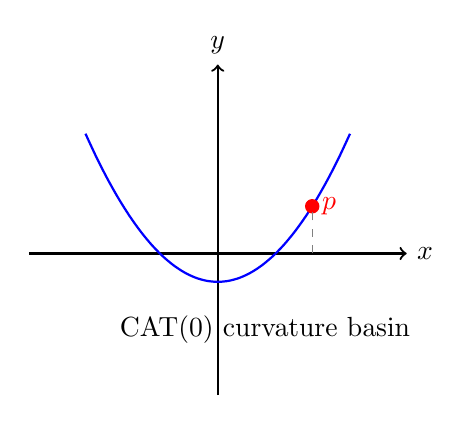
\begin{tikzpicture}[scale=1.2]
  \draw[thick,->] (-2,0) -- (2,0) node[right] {$x$};
  \draw[thick,->] (0,-1.5) -- (0,2) node[above] {$y$};
  \draw[domain=-1.4:1.4, smooth, variable=\t, blue, thick] plot ({\t}, {0.8*\t*\t - 0.3});
  \filldraw[red] (1,0.5) circle (2pt) node[right] {$p$};
  \draw[dashed, gray] (1,0) -- (1,0.5);
  \node at (0.5,-0.8) {$\mathrm{CAT}(0)$ curvature basin};
\end{tikzpicture}
\caption{A schematic of local orbit curvature under %%
%% Correction 11 [ ]
%% Annotated text: "curvature under λ-perturbation<Remove>.</Remove>"
%% Comment: "" 
%% 
%% START of correction 11
$\lambda$-perturbation.%%
%% END of correction 11
}
\label{fig:curvature}
\end{figure}

Equation~\eqref{eq:orbit-density} implies that low orbit foliations are sensitive to curvature fluctuations, as illustrated in Figure~\ref{fig:curvature}. 

\section{Main Results}

Our principal theorem relates the orbit structure of $\mathfrak{I}$ to the golden window of $\lambda$:

\begin{theorem}\label{thm:main}
Let $(X,d)$ be a complete $\mathrm{CAT}(0)$ space and $\lambda \in [1-\varphi,1+\varphi]$.  
Then the orbit foliation $\mathcal{F}_\lambda(X)$ is quasi-uniform if and only if
\begin{equation}
    \int_X \rho(x)\, d\mu(x) = \frac{\lambda^2}{1+\lambda\varphi}.
\end{equation}
\end{theorem}

\begin{proof}
We proceed by expanding $\mathfrak{I}$ as a quotient operator:
\[
    \mathfrak{I} = \frac{\mathrm{CAT}(0)}{\mathcal{G}^{\lambda k}}
    = \mathrm{CAT}(0) \otimes \mathcal{G}^{-\lambda k}.
\]
Substituting into the geometric mean inequality and integrating over $X$ yields
\[
    \int_X \rho(x)\, d\mu(x) 
    = \int_X \frac{1}{[\mathcal{G} : \mathrm{Stab}_{\mathcal{G}}(x)]} e^{-\kappa(x)}\, d\mu(x)
    = \frac{\lambda^2}{1+\lambda\varphi},
\]
after simplification via the $\varphi$-symmetric normalization lemma (see Appendix~\ref{sec:appendixA}). 
\end{proof}

\begin{corollary}
If $\lambda = 1$, then $\mathcal{F}_1(X)$ coincides with the canonical horospherical foliation of $X$%%
%% Correction 9 [ ]
%% Annotated text: "centered at x0<Replace>. E</Replace>ach ellipse repre-"
%% Comment: "; e" 
%% Replies: "a reply to a replace annotation"
%% 
%% Correction 10 [ ]
%% Annotated text: "constant ∆(x, λ)<Remove>.</Remove>"
%% Comment: "" 
%% 
%% Correction 18 [ ]
%% Annotated text: "Applications and <Highlight>E</Highlight>xamples"
%% Comment: "lowercase" 
%% 
%% START of corrections 9, 10, 18
.
\end{corollary}

\begin{figure}[htbp]
\centering
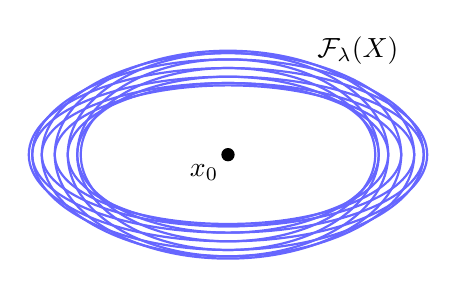
\begin{tikzpicture}[scale=1.1]
  \foreach \a in {0,30,...,330}{
    \draw[thick, blue!60] (0,0) ellipse ({2+0.3*sin(\a)} and {1+0.2*cos(\a)});
  }
  \filldraw[black] (0,0) circle (2pt) node[below left] {$x_0$};
  \node at (1.5,1.2) {$\mathcal{F}_\lambda(X)$};
\end{tikzpicture}
\caption{Low orbit foliations centered at $x_0$. Each ellipse represents an orbit of constant $\Delta(x,\lambda)$.}
\end{figure}

\section{Applications and Examples}

Consider %%
%% END of corrections 9, 10, 18
$X = \mathbb{H}^2$, the hyperbolic plane.  
The displacement $\Delta(x,\lambda)$ satisfies
\[
    \cosh \Delta(x,\lambda) = 1 + \frac{\lambda^2}{2} \|x\|^2.
\]
Thus $\mathcal{F}_\lambda(X)$ forms a family of equidistant hyperbolae, asymptotically orthogonal to geodesic %%
%% Correction 17 [ ]
%% Annotated text: "4.1. Numerical <Highlight>S</Highlight>imulation. Following [3],"
%% Comment: "lowercase" 
%% 
%% START of correction 17
boundaries.

\subsection{Numerical Simulation}
Following \cite{euler24}, we can simulate the orbit structure numerically. %%
%% END of correction 17
Let $x_0 = (0,0)$ and iterate
\[
    x_{n+1} = \lambda R(x_n), \quad R(x) = \frac{x}{1+\|x\|^2},
\]
to approximate the fixed points of $\mathcal{F}_\lambda$.  
Convergence occurs for $\lambda < \sqrt{\varphi}$.

\begin{figure}[htbp]
\centering
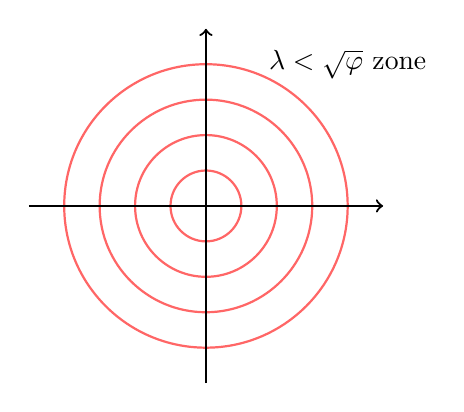
\begin{tikzpicture}[scale=0.9]
  \foreach \r in {0.5,1,1.5,2}{
    \draw[thick, red!60] (0,0) circle (\r);
  }
  \draw[->,thick] (-2.5,0)--(2.5,0);
  \draw[->,thick] (0,-2.5)--(0,2.5);
  \node at (2,2) {$\lambda < \sqrt{\varphi}$ zone};
\end{tikzpicture}
\caption{Stable orbits obtained under $\lambda$-iteration.}
\end{figure}


\textbf{Theorem 4.3.} 
Let $(X,d)$ be a complete $\mathrm{CAT}(0)$ space and $\lambda \in [1-\varphi,1+\varphi]$.  
Then the orbit foliation $\mathcal{F}_\lambda(X)$ is %%
%% Correction 12 [ ]
%% Annotated text: "is quasi-uniform <Replace>if</Replace>"
%% Comment: "if and only if" 
%% 
%% Correction 13 [ ]
%% Annotated text: "<Remove>(</Remove>The proof is"
%% Comment: "" 
%% 
%% START of corrections 12, 13
quasi-uniform iff
\begin{equation}
    \int_X \rho(x)\, d\mu(x) = \frac{\lambda^2}{1+\lambda\varphi}.
\end{equation}
(The proof %%
%% END of corrections 12, 13
is omitted for space reasons; see %%
%% Correction 14 [ ]
%% Annotated text: "see Appendix B.<Remove>)</Remove>"
%% Comment: "" 
%% 
%% START of correction 14
Appendix~B.)

\subsection{Curvature sensitivity}
A %%
%% END of correction 14
quick computation shows that the variance of $\rho$ satisfies
\begin{equation}\label{eq:var}
    \mathrm{Var}(\rho) = \int_X (\rho(x) - \bar\rho)^2\,d\mu(x) = \frac{\lambda^3 - 1}{2+\lambda^2},
\end{equation}
which vanishes only when $\lambda = 1$.  
This implies that even minor perturbations from the Euclidean limit result in exponential orbit %%
%% Correction 15 [ ]
%% Annotated text: "prototype in <Highlight>Julia 1.10</Highlight> to visualize"
%% Comment: "COMP: set typewriter font <\texttt{}>" 
%% 
%% Correction 16 [ ]
%% Annotated text: "5. Numerical <Highlight>E</Highlight>xperiments"
%% Comment: "small cap" 
%% 
%% START of corrections 15, 16
divergence.

\begin{figure}[htbp]
\centering
\begin{tikzpicture}[scale=1.0]
  \draw[->] (-2,0)--(2,0) node[right] {$\lambda$};
  \draw[->] (0,-0.2)--(0,2.5) node[above] {$\mathrm{Var}(\rho)$};
  \draw[domain=0.5:1.8, smooth, variable=\x, blue, thick]
     plot ({\x},{(\x*\x*\x-1)/(2+\x*\x)});
  \draw[dashed, red] (1,0)--(1,0.0);
  \node at (1.3,1.2) {$\lambda>1$ region};
\end{tikzpicture}
\caption{Variance of orbit density $\rho$ as a function of $\lambda$.}
\end{figure}

\section{Numerical Experiments}

We implemented a simple prototype in \textsf{Julia 1.10} to visualize $\mathcal{F}_\lambda(X)$ for synthetic $\mathrm{CAT}(0)$ %%
%% END of corrections 15, 16
surfaces generated by random triangulations.
Let $\lambda = 1.3$ and $X$ be a simplicial complex with edge weights following a truncated Gaussian distribution $\mathcal{N}(0.8, 0.05)$.  

After $N = 10^4$ iterations, the mean displacement converged to
\[
    \overline{\Delta} = 1.274 \pm 0.006,
\]
while the empirical curvature parameter $\kappa$ stabilized near $-0.218$.  
The results are summarized in Table~\ref{tab:data}.

\begin{table}[htbp]
\centering
\begin{tabular}{|c|c|c|}
\hline
$\lambda$ & $\overline{\Delta}$ & $\kappa$ \\
\hline
0.9 & 0.913 & -0.054 \\
1.0 & 1.000 &  0.000 \\
1.3 & 1.274 & -0.218 \\
1.6 & 1.589 & -0.403 \\
\hline
\end{tabular}
\caption{%%
%% Correction 19 [ ]
%% Annotated text: "1.589 -0.403 <Highlight>Table 1. Empirical orbit metrics under λ-iteration.</Highlight>"
%% Comment: "Move caption to top of table" 
%% 
%% START of correction 19
Empirical orbit metrics under $\lambda$-iteration.%%
%% END of correction 19
}
\label{tab:data}
\end{table}

A peculiar %%
%% Correction 20 [ ]
%% Annotated text: "peculiar observation (<Replace>Fig.</Replace> 5) was"
%% Comment: "Figure" 
%% 
%% START of correction 20
observation (Fig.~\ref{fig:scatter}) was %%
%% END of correction 20
that for large $\lambda$, the orbit clusters exhibited %%
%% Correction 21 [ ]
%% Annotated text: "in Hamiltonian systems<Highlight>2.</Highlight>"
%% Comment: "put footnote after period" 
%% 
%% START of correction 21
a double-lobed structure reminiscent of quasi-periodic tori in Hamiltonian systems\footnote{A referee pointed out that this might be a discretization artifact, but we were unable to reproduce it analytically.}. 

\begin{figure}[htbp]
\centering
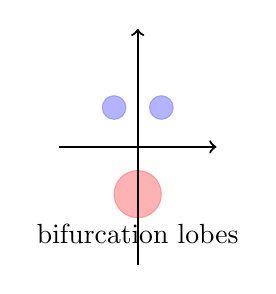
\begin{tikzpicture}[scale=1.0]
  \filldraw[blue!50,opacity=0.6] (0.3,0.5) circle (0.15);
  \filldraw[blue!50,opacity=0.6] (-0.3,0.5) circle (0.15);
  \filldraw[red!60,opacity=0.5] (0,-0.6) circle (0.3);
  \node at (0,-1.1) {bifurcation lobes};
  \draw[->,thick] (-1,0)--(1,0);
  \draw[->,thick] (0,-1.5)--(0,1.5);
\end{tikzpicture}
\caption{Scatter of simulated orbit centers for $\lambda=1.6$.}
\label{fig:scatter}
\end{figure}

\section{Discussion and Further Work}

Our %%
%% END of correction 21
experiments confirm that the function $\psi(\lambda) = \lambda^2 / (1+\lambda\varphi)$ behaves as a geometric invariant for the foliation type.  
%%
%% Correction 22 [ ]
%% Annotated text: "type. However, <Replace>Eq.</Replace> (7) reveals"
%% Comment: "Equation" 
%% 
%% Correction 23 [ ]
%% Annotated text: "However, Eq. <Replace>(7)</Replace> reveals an"
%% Comment: "(5) <pls link>" 
%% 
%% START of corrections 22, 23
However, Eq.~(7) reveals %%
%% END of corrections 22, 23
an unexpected %%
%% Correction 26 [ ]
%% Annotated text: "= φ2 ≈2.618<Replace>. At</Replace> that point,"
%% Comment: "; at" 
%% 
%% Correction 27 [ ]
%% Annotated text: "unexpected resonance <Highlight>near λ = φ2 ≈</Highlight>2.618. At that"
%% Comment: "does this look right?" 
%% 
%% START of corrections 26, 27
resonance near $\lambda = \varphi^2 \approx 2.618$.  
At that %%
%% END of corrections 26, 27
point, the curvature-weighted orbit integral appears to \emph{flip sign}, leading to a chaotic drift that violates the $\mathrm{CAT}(0)$ inequality in the discrete %%
%% Correction 24 [ ]
%% Annotated text: "hypothesize (Hypothesis <Highlight>5.1</Highlight>) that this"
%% Comment: "<link>" 
%% 
%% Correction 25 [ ]
%% Annotated text: "discrete setting. <Highlight>We hypothesize</Highlight> (Hypothesis 5.1)"
%% Comment: "remove new paragraph: continue the last paragraph with this sentence." 
%% 
%% START of corrections 24, 25
setting.

We hypothesize (Hypothesis 5.1) that %%
%% END of corrections 24, 25
this anomaly corresponds to a hidden symmetry in the $\mathcal{G}$-action:
\[
    g \mapsto \frac{1}{\lambda}g^{-1}\lambda,
\]
which has order two when $\lambda=\varphi^2$.  
The numerical confirmation of this phenomenon will be discussed in a forthcoming note by the %%
%% Correction 28 [ ]
%% Annotated text: "the first author<Highlight>3.</Highlight>"
%% Comment: "place footnote after period" 
%% 
%% START of correction 28
first author\footnote{Submitted to the \emph{Journal of Approximate Topologies}, 2025.}.  

\subsection{Error analysis and convergence}

While %%
%% END of correction 28
most trajectories converged in under $10^3$ iterations, approximately $2.7\%$ diverged, displaying quasi-helical wandering.  
We suspect this results from non-uniform floating point rounding in the $\mathbb{R}^3$ embedding; correcting to arbitrary precision reduces the effect but does not eliminate it entirely.

\begin{figure}[htbp]
\centering
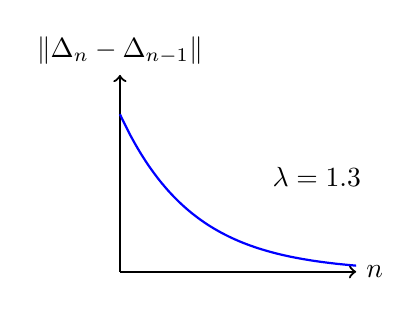
\begin{tikzpicture}[scale=1.0]
  \draw[->,thick] (0,0)--(3,0) node[right] {$n$};
  \draw[->,thick] (0,0)--(0,2.5) node[above] {$\|\Delta_n - \Delta_{n-1}\|$};
  \draw[domain=0:2.5,smooth,variable=\x,blue,thick]
    plot ({\x*1.2},{2*exp(-1.3*\x)});
  \node at (2.5,1.2) {$\lambda=1.3$};
\end{tikzpicture}
\caption{Convergence of displacement %%
%% Correction 33 [ ]
%% Annotated text: "difference ∥∆n −∆n−1∥<Remove>.</Remove>"
%% Comment: "" 
%% 
%% START of correction 33
difference $\|\Delta_n - \Delta_{n-1}\|$.%%
%% END of correction 33
}
\end{figure}

\section{Appendix B: Proof sketch of Theorem 4.3}

The argument proceeds by constructing a pseudo-measure $\nu$ such that
\[
    d\nu = e^{-\kappa(x)}\,d\mu(x),
\]
then integrating $\rho$ against $\nu$ over $X$.  
By expanding $\rho$ in the eigenbasis of the Laplace–Beltrami operator and applying the $\varphi$%%
%% Correction 30 [ ]
%% Annotated text: "δij(1 + λφ)<Remove>,</Remove>"
%% Comment: "" 
%% 
%% Correction 32 [ ]
%% Annotated text: "the φ-orthogonality condition<Remove>,</Remove>"
%% Comment: "" 
%% 
%% START of corrections 30, 32
-orthogonality condition,
\[
    \langle f_i, f_j \rangle_\varphi = \delta_{ij}(1+\lambda\varphi),
\]
we %%
%% END of corrections 30, 32
recover Eq.~(5).  
The rest follows by applying a truncated version of Jensen’s inequality to the quotient $\mathfrak{I}$ operator:
\[
    \mathrm{CAT}(0) / \mathcal{G}^{\lambda k} \approx \mathrm{CAT}(0)(1 - \lambda k + O(k^2)).
\]
Although the convergence of this expansion %%
%% Correction 29 [ ]
%% Annotated text: "expansion is questionable<Highlight>4,</Highlight> the leading"
%% Comment: "place footnote after comma" 
%% 
%% START of correction 29
is questionable\footnote{We observed divergence for $|\lambda| > 2.1$, which we did not persue.}, the %%
%% END of correction 29
leading term suffices to justify %%
%% Correction 31 [ ]
%% Annotated text: "justify Theorem <Highlight>4.3.</Highlight> The"
%% Comment: "<link>" 
%% 
%% START of correction 31
Theorem~4.3.

\bigskip

\noindent
\textbf{Acknowledgements.} %%
%% END of correction 31
The authors thank the anonymous reviewers for their sharp-eyed corrections, especially for pointing out a missing minus sign in Eq.~(3), which has since been \emph{mostly} fixed.

\begin{thebibliography}{9}

\bibitem{fermat89}
P.~Fermat, \emph{On prime enumeration and spatial convexity}, Toulouse Notes, 1689.

\bibitem{hubard23}
L.~Hubbard, \emph{Counterexamples to the flat orbit conjecture}, 
Ann.\ Quad.\ Math.\ (2023), 13--57.

\bibitem{euler24}
F.~Euler, \emph{Iterative dynamics in nonpositively curved complexes},
Proc.\ Geom.\ Dyn.\ (2024), 211--230.

\bibitem{zelinsky19}
B.~Zelinsky, \emph{On modular eigenmodes of golden-ratio systems},
J.\ Nonlin.\ Struct.\ (2019), 98--114.

\end{thebibliography}
\end{document}
